%%%%%%%%%%%%%%%%%%%%%%%%%%%%%%%%%%%%%%%%%%%%%%%%%%%%%
%
%  Template
%  Beamer Presentation by Chris Bourke
%
%%%%%%%%%%%%%%%%%%%%%%%%%%%%%%%%%%%%%%%%%%%%%%%%%%%%%%%%%%%%%%%%%%%%%%%

\documentclass[]{beamer}
%\documentclass[handout]{beamer}

\geometry{papersize={16cm,9cm}}

% For handout version:
%\usetheme[hideothersubsections,slidenumbers]{UNLTheme}
\usetheme[hideothersubsections]{UNLTheme}
\usepackage{amssymb}
\input{StandardCommands}
\usepackage[linesnumbered,ruled,vlined]{algorithm2e}
\SetKwComment{Comment}{//}{}
\DontPrintSemicolon
\SetKwSty{textsc} %
%\SetAlFnt{\scriptsize} %
\SetKwInOut{Input}{Input} %
\SetKwInOut{Output}{Output} %
%\setalcapskip{1em} % changed to
\SetAlCapSkip{1em}
\setlength{\algomargin}{2em} %
%\Setvlineskip{0em} % changed to:
\SetVlineSkip{0em}

\usepackage{tikz}
\usetikzlibrary{fadings}
\usetikzlibrary{shapes.geometric,shapes.symbols}
\usetikzlibrary{calc,shapes.multipart,chains,arrows}
\usetikzlibrary{arrows.meta,calc,shapes.multipart,chains,arrows}
%\usetikzlibrary{calc,shapes.multipart,chains,arrows}
%%\usetikzlibrary{backgrounds}
\usetikzlibrary{backgrounds}
\usetikzlibrary{decorations.pathreplacing}
\usetikzlibrary{decorations.pathmorphing}
\tikzset{onslide/.code args={<#1>#2}{%
  \only<#1>{\pgfkeysalso{#2}} % \pgfkeysalso doesn't change the path
}}
\tikzset{temporal/.code args={<#1>#2#3#4}{%
  \temporal<#1>{\pgfkeysalso{#2}}{\pgfkeysalso{#3}}{\pgfkeysalso{#4}} % \pgfkeysalso doesn't change the path
}}

\tikzset{
    fading speed/.code={
        \pgfmathtruncatemacro\tikz@startshading{50-(100-#1)*0.25}
        \pgfmathtruncatemacro\tikz@endshading{50+(100-#1)*0.25}
        \pgfdeclareverticalshading[%
            tikz@axis@top,tikz@axis@middle,tikz@axis@bottom%
        ]{axis#1}{100bp}{%
            color(0bp)=(tikz@axis@bottom);
            color(\tikz@startshading)=(tikz@axis@bottom);
            color(50bp)=(tikz@axis@middle);
            color(\tikz@endshading)=(tikz@axis@top);
            color(100bp)=(tikz@axis@top)
        }
        \tikzset{shading=axis#1}
    }
}

\usepackage{multirow}
\usepackage{multicol}

\definecolor{steelblue}{rgb}{0.2745,0.5098,0.7059}
\hypersetup{
    colorlinks = true,
    urlcolor = {steelblue},
    linkbordercolor = {white}
}

\definecolor{mintedBackground}{rgb}{0.95,0.95,0.95}
\definecolor{mintedInlineBackground}{rgb}{.90,.90,1}

%\usepackage{newfloat}
\usepackage{minted}
\setminted{mathescape,
               linenos,
               autogobble,
               frame=none,
               fontsize=\small,
               framesep=2mm,
               framerule=0.4pt,
               %label=foo,
               xleftmargin=2em,
               xrightmargin=0em,
               startinline=true,  %PHP only, allow it to omit the PHP Tags *** with this option, variables using dollar sign in comments are treated as latex math
               numbersep=10pt, %gap between line numbers and start of line
               style=default, %syntax highlighting style, default is "default"
               			    %gallery: http://help.farbox.com/pygments.html
			    	    %list available: pygmentize -L styles
               bgcolor=mintedBackground} %prevents breaking across pages
               
\setmintedinline{bgcolor={mintedInlineBackground}}
\setminted[text]{bgcolor={},linenos=false,autogobble,xleftmargin=1em}

\tikzstyle{decision} = [diamond, draw, fill=yellow!20, 
    text width=6em, text badly centered, node distance=5cm, inner sep=0pt]
\tikzstyle{block} = [rectangle, draw, fill=blue!20, 
    text width=5em, text centered, node distance=5cm, minimum height=4em]
\tikzstyle{action} = [rectangle, draw, fill=green!20, 
    text width=5em, text centered, rounded corners, node distance=5cm, minimum height=4em]
\tikzstyle{line} = [draw, -latex']

\title[~]{Computer Science I}
\subtitle{Loops}
\author[~]{Dr.\ Chris Bourke\\ \email{cbourke@cse.unl.edu}} %
\date{~}

\begin{document}

\begin{frame}
  \titlepage
\end{frame}

\setbeamertemplate{section in toc}{\inserttocsectionnumber.~\inserttocsection}
\setbeamercolor{section in toc}{fg=black}
%\setbeamertemplate{subsection in toc}{~} %\inserttocsubsection\\}

\begin{frame}
  \frametitle{Outline}
%{\footnotesize
%\begin{NoHyper}
%  \tableofcontents[hideallsubsections]
%\end{NoHyper}
%}

\setbeamercolor{enumerate item}{bg=white,fg=black}
\setbeamercolor{item}{bg=white,fg=black}
\setbeamercolor{item projected}{bg=white,fg=black}
\setbeamercolor{enumerate subitem}{fg=red!80!black}
\setbeamertemplate{enumerate items}[default]
\begin{enumerate}
  \item Introduction
  \item For loops %include increment operators
  \item While loops %include discussion on when to use
  \item Other Loops \& Issues 
  \item Pitfalls
  \item Exercises
\end{enumerate}

\end{frame}

\section{Introduction}

\begin{frame}
    \frametitle{}
    \framesubtitle{}
    
    \begin{center}
    {\Huge Part I: Introduction}\\
    {\Large Motivation \& Introduction to Loop Control Structures}
    \end{center}

\end{frame}


\begin{frame}
  \frametitle{Motivation}

  \begin{itemize}[<+->]
    \item Need a way to \emph{repeatedly} execute a block of code
    \item Process data: apply an operation to each piece of data
    %element in an array (sum numbers, print them, insert them into a table, etc.)
    \item Repeat an operation until some condition is satisfied
  \end{itemize}

\end{frame}

\begin{frame}
  \frametitle{Loops}

  \begin{itemize}[<+->]
    \item A \emph{loop} allows us to \emph{repeatedly} execute a 
      block of code while some \emph{condition} is satisfied
    \item While some boolean expression or condition evaluates to true, the loop will continue to execute
    \item Once the condition is no longer satisfied, the loop 
      \emph{terminates} its execution
    \item Each time a loop executes is referred to as an \emph{iteration}
    \item Different types of loops      
    \item Components of a loop
  \end{itemize}
    
\end{frame}

\begin{frame}
  \frametitle{Loop Components}

  A loop has several main components:
  \begin{enumerate}[<+->]
    \item An initialization statement -- a statement that indicates how the loop \emph{begins}
    \item A continuation condition -- a boolean statement that specifies 
    whether the loop should continue executing
    \item An iteration statement -- a statement that makes progress toward the termination of
    	the loop
    \item Loop Body -- the block of code that gets executed for each \emph{iteration}
  \end{enumerate}

\onslide<5->{
\emph{Termination Condition} -- negation of the continuation condition
} 
\end{frame}

\begin{frame}
  \frametitle{Simple Example}
  
  Printout numbers 1 through 10:
  \begin{enumerate}
    \item Initialize a variable $i$ to 1
    \item While the variable $i$'s value is less than or equal to 10\ldots
    \item Print $i$
    \item Increment $i$ by adding 1 to it
    \item Go to step 2
  \end{enumerate}

\end{frame}

\begin{frame}
  \frametitle{Flow Diagram}
  \framesubtitle{}
  
\begin{center}  
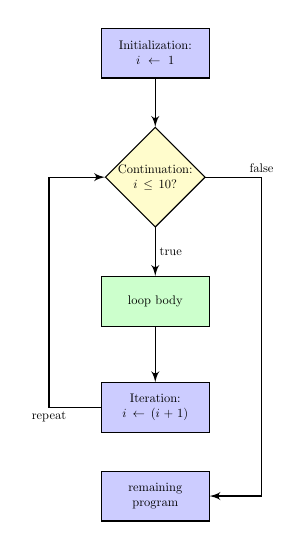
\begin{tikzpicture}[node distance=1cm,auto,scale=0.45,transform shape]

    \node [block,text width=8em] (a) {Initialization: $i \leftarrow 1$};
    \node [decision,node distance=3.5cm,text width=6em,text centered, below of=a] (decide) {Continuation: $i \leq 10$?};
    \node [block,node distance=3.5cm,text width=8em, fill=green!20, below of=decide] (body) {loop body};
    \node [block,node distance=3.0cm,text width=8em, below of=body] (c) {Iteration: $i \leftarrow (i + 1)$};
    \node[block,node distance=2.5cm,text width=8em,below of=c] (d) {remaining program};
    
    % Draw edges
    \path [line] (a) -- (decide);
    \path [line] (body) -- (c);
    %\path [line] (c) -- (d);
    \path [line] (decide) -- node {true} (body);
    \path [line] (c)   --++  (-3,0) node[below] {repeat} |- (decide);
    \path [line] (decide)   --++  (3,0) node [above] {false} |- (d);


\end{tikzpicture}
\end{center}

\end{frame}
 
\section{For Loops}

\begin{frame}
    \frametitle{}
    \framesubtitle{}
    
    \begin{center}
    {\Huge Part II: For Loops}\\
    {\Large ~}
    \end{center}

\end{frame}


\begin{frame}[fragile]
  \frametitle{For Loop}
  \framesubtitle{}

\begin{itemize}[<+->]
  \item A a \emph{for loop} uses the keyword \mintinline{c}{for} 
  \item All three elements: initialization, continuation and increment are 
  \begin{itemize}
    \item placed on the same line
    \item enclosed within parentheses
  \end{itemize}
  \item Loop body is denoted using curly brackets
\end{itemize}

\end{frame}


\begin{frame}[fragile]
  \frametitle{For Loop}
  \framesubtitle{}
  
\begin{minted}{c}
int i;
for(i=1; i<=10; i++) {
  printf("i = %d\n", i);
}  
\end{minted}

\begin{itemize}[<+(1)->]
  \item Initialization, executed only once before the loop begins
  \item Continuation condition, evaluated before each iteration
  \item Iteration executed at the end of each loop
  \item New syntax: \mintinline{c}{i++}
  \item Loop body denoted with curly brackets
  \item Correct usage of semicolons
  \item Style elements
  \item Demonstration %http://pythontutor.com/c.html#mode=edit
\end{itemize}

\end{frame}


\subsection{Increment Operators}

\begin{frame}[fragile]
  \frametitle{Increment Operators}
  \framesubtitle{}

Several common ``short-hand'' operators for increment/decrement:  
\begin{itemize}[<+(1)->]
  \item \mintinline{c}{i++} adds 1 to the variable \mintinline{c}{i}
  \item \mintinline{c}{i--} subtracts 1 from the variable \mintinline{c}{i}
  \item ``Equivalent'' to \mintinline{c}{i = i + 1} and \mintinline{c}{i = i - 1}
%syntactic sugar overlay
  \item Honorable mention: prefix versions \mintinline{c}{++i} and \mintinline{c}{--i}  
\end{itemize}
\end{frame}

\begin{frame}[fragile]
  \frametitle{More Increment Operators}
  \framesubtitle{}

You can also use compound increment operators:
\begin{itemize}[<+(1)->]
  \item \mintinline{c}{a += 10;} adds 10 to the variable \mintinline{c}{a}
  \item \mintinline{c}{a -= 5;} subtracts 5 from the variable \mintinline{c}{a}
  \item \mintinline{c}{a *= 2;} multiplies \mintinline{c}{a} by 2
  \item \mintinline{c}{a /= 3;} divides \mintinline{c}{a} by 3
\end{itemize}
  
\end{frame}


\begin{frame}[fragile]
  \frametitle{More Examples}
  \framesubtitle{}
  
\begin{minted}{c}
//print numbers 10, 20, 30, ... 100
int i;
for(i=10; i<=100; i+=10) {
  printf("%d\n", i);
}
printf("%d\n", i); 

int n = 10;
int sum = 0; //without initialization, no default value
for(i=1; i<n; i++) {
  //sum = sum + i;
  sum += i;
}
printf("sum of integers 1..%d = %d\n", n, sum);
\end{minted}

\end{frame}

\section{While Loops}

\begin{frame}
    \frametitle{}
    \framesubtitle{}
    
    \begin{center}
    {\Huge Part III: While Loops}\\
    {\Large ~}
    \end{center}

\end{frame}


\begin{frame}
  \frametitle{While Loops}
  \framesubtitle{}

\begin{itemize}[<+->]
  \item A a \emph{while loop} uses the keyword \mintinline{c}{while} 
  \item Three elements (initialization, continuation, increment) are not on the same line
  \item Same behavior: continuation condition is checked at the start of the loop
\end{itemize}

\end{frame}


\begin{frame}[fragile]
  \frametitle{While Loops}
  \framesubtitle{}

\begin{minted}{c}
int i = 1; 
while(i <= 10) {
  printf("i = %d\n", i);
  i++;
}
\end{minted}


\begin{itemize}[<+(1)->]
  \item Initialization is before and outside the loop structure
  \item \mintinline{c}{while} statement contains only the continuation condition
  \item Increment is done \emph{inside} the loop body
  \item Take care: order inside the loop matters
\end{itemize}

\end{frame}


\begin{frame}[fragile]
  \frametitle{While Loops}
  \framesubtitle{}

\begin{minted}{c}
int i = 1; 
while(i <= 10) {
  i++;
  printf("i = %d\n", i);
}
\end{minted}

\end{frame}


\begin{frame}[fragile]
  \frametitle{Why Multiple Loops?}
  \framesubtitle{}

Why do we have multiple loop control structures?
\begin{itemize}[<+(1)->]
  \item Any for loop can be rewritten as a while loop and vice versa
  \item Syntactic sugar, flexibility, variety
  \item Generally, the situation/context will inform how ``natural'' each loop is
  \item Use for loops when the number of iterations is known up front 
  %(ie a fixed number of times or n times, where n is a known variable)
  \item Use while loops when you don't know how many iterations will be executed/they may vary depending on the variable values
\end{itemize}

\end{frame}


\begin{frame}[fragile]
  \frametitle{While Loop Scenario}
  \framesubtitle{}

Example: write a loop (or loops) to \emph{normalize} a number:
  $$89237.49283 \rightarrow 8.923749283 \times 10^{4}$$
  $$321.321 \rightarrow 3.21321 \times 10^{2}$$
  $$0.00432 \rightarrow 4.32 \times 10^{-3}$$

\end{frame}


\begin{frame}[fragile]
  \frametitle{While Loop Scenario}
  \framesubtitle{}

\begin{minted}{c}
  double x = 89237.49283;
  int counter = 0;
  while(x > 10) {
    x /= 10.0;
    counter++;
  }
  printf("x = %f * 10^%d\n", x, counter);
  while(x < 1) {
    x *= 10.0;
    counter--;
  }
  printf("x = %f * 10^%d\n", x, counter);
  return 0;
\end{minted}
\end{frame}

\section{Other Loops}

\begin{frame}
    \frametitle{}
    \framesubtitle{}
    
    \begin{center}
    {\Huge Part IV: Other Issues \& Types of Loops}\\
    {\Large ~}
    \end{center}

\end{frame}

\begin{frame}[fragile]
  \frametitle{Loop Variable Scoping}
  \framesubtitle{}

\begin{itemize}[<+->]
  \item For loop examples declared the iteration variable before the loop
\begin{minted}{c}
int i;
for(i=0; i<=10; i++) {
  ...
}
\end{minted}  
  \item The \emph{scope} of \mintinline{c}{i} lasted after the loop
\end{itemize}

\end{frame}

\begin{frame}[fragile]
  \frametitle{Loop Variable Scoping}
  \framesubtitle{}

\begin{itemize}[<+->]
  \item Many modern languages and newer versions of C (C99) allow a loop-scoped
  variable declaration:
\begin{minted}{c}
for(int i=0; i<=10; i++) {
  ...
}
\end{minted}  
  \item Scope of \mintinline{c}{i} is limited to the loop
  \item If you use this modern style, you must compile with: \\
  \mintinline{text}{gcc -std=c99} or \\
  \mintinline{text}{c99}
\end{itemize}
\end{frame}

\begin{frame}[fragile]
  \frametitle{Flag-Controlled Loops}
  \framesubtitle{}

\begin{itemize}[<+->]
  \item Instead of a continuation condition, we could use a boolean ``flag'' variable
  \item Most commonly used with while loops
\begin{minted}[fontsize=\scriptsize]{c}
int flag = 1;
while(flag) {
  ...
  if(<some complex logic>) {
    flag = 0;
  }
}
\end{minted}
  \item Sometimes, people use \mintinline{c}{break} to break out instead:
\begin{minted}[fontsize=\scriptsize]{c}
while(1) {
  ...
  if(<some complex logic>) {
    break;
  }
}
\end{minted}
\end{itemize}
\end{frame}

 
\begin{frame}[fragile]
  \frametitle{Do-While Loops}
  \framesubtitle{}

\begin{itemize}[<+->]
  \item Do-while loops check the continuation condition at the \emph{end} of the loop
  \item Consequence: they always execute \emph{at least once}
  \item Example:
\begin{minted}{c}
int i = 0;
do {
  i++;
  print("i = %d\n", i);
} while(i < 10);
\end{minted}
\end{itemize}

\end{frame}

\begin{frame}[fragile]
  \frametitle{For Each Loops}
  \framesubtitle{}


\begin{itemize}[<+->]
  \item Many languages support ``for each'' loops
  \item Used to iterate over ``collections'' (arrays, sets, lists, etc.)
  \item Not supported in C
\end{itemize}
  
  
\end{frame}

\begin{frame}[fragile]
  \frametitle{Nesting Loops}
  \framesubtitle{}

\begin{itemize}[<+->]
  \item Loops can be written inside of other loops
  \item Called ``nesting'' or \emph{nested loops}
  \item Very common when iterating over matrices/tables of data 
  \item For each row, then for each column in the row
  \item Example:
\begin{minted}{c}
int i, j;
for(i=1; i<=10; i++) {
  for(j=1; j<=10; j++) {
    printf("%d\n", (i+j));
  }
}
\end{minted}
\end{itemize}

\end{frame}
 
\section{Pitfalls}

\begin{frame}
    \frametitle{}
    \framesubtitle{}
    
    \begin{center}
    {\Huge Part V: Pitfalls}\\
    {\Large Common Errors \& Misconceptions}
    \end{center}

\end{frame}


\begin{frame}[fragile]
  \frametitle{Pitfall}
  \framesubtitle{Improper Increment}

Consider the following code:
\begin{minted}{c}
int i = 1;
while(i <= 10) {
  printf("%d\n", i);
}
\end{minted}

\begin{itemize}[<+(1)->]
  \item Results in an infinite loop
  \item There is no increment/progress toward the termination condition 
  \item To kill a command line program: control-C
\end{itemize}

\end{frame}


\begin{frame}[fragile]
  \frametitle{Pitfall}
  \framesubtitle{Misplaced Semicolon}

Consider the following code:
\begin{minted}{c}
int i = 1;
while(i <= 10); {
  printf("%d\n", i);
  i++;
}
\end{minted}

\begin{itemize}[<+(1)->]
  \item Results in an infinite loop
  \item Extraneous semicolon, similar to conditional pitfall
  \item Empty loop body
\end{itemize}

\end{frame}


\begin{frame}[fragile]
  \frametitle{Pitfall}
  \framesubtitle{Bad Coding Style}
  
Consider the following code:
\begin{minted}{c}
int i = 1;
while(i <= 10)
  printf("%d\n", i);
  i++;
\end{minted}

\begin{itemize}[<+(1)->]
  \item Results in an infinite loop
  \item Missing brackets means loop body is \emph{only the next line}
  \item Always include curly brackets even if they are not necessary!
\end{itemize}

\end{frame}


\begin{frame}[fragile]
  \frametitle{Pitfall}
  \framesubtitle{Off-By-One Errors}

\begin{itemize}[<+->]
  \item Initialization/continuation must be considered carefully
  \item Loops may be off-by-one iteration (start or end)
  \item Zune Bug: December 31st, 2008
  \item Thousands of Zunes froze for 24 hours
  \item 2008 was a leap year: 366 days
  \item An embedded module in the Zune contained the following
          (actual) code
\end{itemize}

\end{frame}

\begin{frame}[fragile]
  \frametitle{Zune Bug}
  \framesubtitle{What happened?}

\begin{minted}{c}
while(days > 365) {
  if(IsLeapYear(year)) {
    if(days > 366) {      
      days -= 366;
      year += 1;
    }
  } else {
    days -= 365;
    year += 1;
  }
}
\end{minted}

\end{frame}

 
\section{Exercises}

\begin{frame}
    \frametitle{}
    \framesubtitle{}
    
    \begin{center}
    {\Huge Part VI: Exercises}\\
    {\Large ~}
    \end{center}

\end{frame}

\begin{frame}[fragile]
  \frametitle{Exercise}
  \framesubtitle{}

Write code snippets to do the following.

\begin{enumerate}
  \item Print a list of even integers 0 to $n$, one to a line
  \item The same list, but delimited by commas
  \item A list of integers divisible by 3 between 10 and 100 (print a total as well)
  \item Prints all positive powers of two, $1, 2, 4, 8, \ldots, 2^{30}$
  \item Prints all even integers 2 thru 200 on 10 different lines 
    (10 numbers per line) in reverse order
  \item Prints the following pattern of numbers (hint: use some value of $i+10j$):
\end{enumerate}
\begin{minted}{text}
11, 21, 31, 41, ..., 91, 101
12, 22, 32, 42, ..., 92, 102
...
20, 30, 40, 50, ..., 100, 110
\end{minted}
\end{frame}

\begin{frame}[fragile]
  \frametitle{Exercise}
  \framesubtitle{}

Write a FizzBuzz program: print numbers from 1 to 100, but for numbers
that are multiples of 3 print ``Fizz'' instead.  For numbers that are
multiples of 5, print ``Buzz'' instead.  For numbers that are multiples
of both 3 and 5, print ``FizzBuzz''

\end{frame}

\begin{frame}[fragile]
  \frametitle{Exercise}
  \framesubtitle{}

Implement a program to use the Babylonian method to compute a square 
root of a number $a$ using the series,

$$x_{n+1} = \frac{1}{2} \cdot \left(x_n + \frac{a}{x_n} \right), \quad x_0 = 1$$

\end{frame}

\begin{frame}[fragile]
  \frametitle{Exercise}
  \framesubtitle{}

Example: compute $\sqrt{2}$ ($a = 2$)

\onslide<2->{
$$x_1 = \frac{1}{2} \cdot \left(x_0 + \frac{a}{x_0} \right)$$
}
\onslide<3->{
$$x_1 = \frac{1}{2} \cdot \left(1 + \frac{2}{1} \right) = 1.5$$
}
\onslide<4->{
$$x_2 = \frac{1}{2} \cdot \left(x_1 + \frac{a}{x_1} \right)$$
}
\onslide<5->{
$$x_2 = \frac{1}{2} \cdot \left(1.5 + \frac{2}{1.5} \right) = 1.41666$$
}
\end{frame}

\begin{frame}[fragile]
  \frametitle{Exercise}
  \framesubtitle{}

Would you accept a job with the following conditions?

\begin{itemize}
  \item You only get paid a dollar a month.
  \item However, each month your pay doubles.
  \item Your contract lasts 2 years.
\end{itemize}

Write a program to project your earnings.
\end{frame}

\begin{frame}[fragile]
  \frametitle{Exercise}
  \framesubtitle{}

DogeCoin is 'sploding!  It increases 20\% in value 
every week!  Suppose we start with 1000 DogeCoin
which is initially worth \$10 (1 DogeCoin = 1 cent).
Let's take the following strategy: at the end of
each week, we sell half our gains, and keep the rest
growing.  Then, at the end of the year we'll report
how much cash we have, how much DogeCoin we have, and
how much that is worth in total USD.

\end{frame}



\end{document} 
